\documentclass[UTF8]{ctexart}

\usepackage{mathptmx}
\usepackage{amsfonts,amsmath,amssymb}% AMS-LaTeX 符号、公式
\numberwithin{equation}{section}

\usepackage[a4paper,margin=2.5cm,bottom=2.5cm]{geometry}% 页边距和纸张大小
\usepackage{longtable,multirow,array}% 各种基本的表格宏包
\usepackage{booktabs}% 三线表宏包
\usepackage{enumerate}
\usepackage{pgfplots}% 图表
\usepackage{caption}
\usepackage{float}
\usepackage{footnote}
%\usepackage{tikz}% 函数图像
%\pgfplotsset{width=10cm,compat=1.9}
\tikzset{elegant/.style={smooth,thick,samples=50,cyan}}
\tikzset{eaxis/.style={->,>=stealth}}
%\tikzset{elegant/.style={smooth,thick,samples=50,magenta}}
\newtheorem{Proof}{证明}%[section]
\newtheorem{qiuzheng}{求证}%[section]
\linespread{1.5}
\usepackage{graphicx}
\usepackage{subfigure}

% 设置文献
% \bibliographystyle{unsrt}
\title{《基于深度学习的交通流量预测与优化》\\中期检查报告}

\author{}

\begin{document}

\maketitle

\newpage
\setcounter{page}{1}


\section{项目执行情况}
	\subsection{整体目标和预期进展}
本项目的整体目标是建立一个基于深度学习的高精度、高效率和高鲁棒性的交通流量预测模型,利用历史的区域交通流量数据对下一时刻某一区域的交通流量进行预测,并基于该模型进行简单的初步应用。

项目的整体研究计划包含以下六个阶段:

\begin{itemize}
	\item
	第一阶段:完成对各类神经网络和深度学习框架的学习。
	\item
	第二阶段:查找相关研究和文献资料,研究已有模型的架构与特点,分析各类模型优缺点,进行文献总结整理。
	\item
	第三阶段:搜集原始交通数据,进行预处理,并着手建立模型雏形。
	\item
	第四阶段:分析总结模型缺陷与瓶颈,制定优化方案以进一步完善模型,提升模型性能。
	\item
	第五阶段:建模收尾,可视化实验结果,讨论预测结果潜在价值与模型现实意义
	\item
	第六阶段:选取现实数据集检验模型效果,以研究报告和学术论文等方式总结研究成果
\end{itemize}

根据项目进展安排,到2020年10月,项目至少应达到第三阶段。

	\subsection{中期项目进度}
目前研究进展与计划基本一致,已完成了前三阶段的主要任务,取得的主要进展如下:

\begin{enumerate}
	\def\labelenumi{\arabic{enumi}.}
	\item
	完成了对数十篇交通预测相关文献资料的收集与阅读:
	
	\begin{itemize}
		\item
		了解了时空数据的基本特点与时空预测问题主要任务和难点,以及现有交通预测问题的研究内容,确定了本研究的预测任务和目标。
		\item
		研究了目前相关研究已提出的各类模型的构架和特点,包括传统统计模型、机器学习模型和深度神经网络模型,对各类模型的优缺点进行整理和总结,以启示后续建模工作。
		\item
		重点阅读和学习了现有基于深度神经网络解决交通预测任务的文献,对每个代表性模型选取了一至两篇论文进行了深入的研读和阅读笔记整理。
		\item
		探究了该预测问题上目前的研究瓶颈和不足。
	\end{itemize}
	\item
	初步建立基本模型
	
	基于前述探索性研究,总结了时空数据的基本特征,具体刻画了交通流量预测问题。选择图卷积网络(Graph
	Convolutional Network, GCN)对数据的空间相关性和时间相关性进行建模。
	\item
	实现数据预处理,着手进行模型实验
	
	搜集了可靠的公开数据集并完成数据预处理,着手进行模型实验,检验模型的基本预测效果,并根据实验结果调整模型架构和模型参数。
\end{enumerate}



\section{主要研究进展}

\subsection{提出基于图卷积网络的交通流量预测方法}
交通流量预测任务的核心任务在于从历史交通流量数据中挖掘有价值的信息,得到未来一定时间内特定区域的流量预测值。交通流量数据属于时空数据(spatial temporal data),是具有空间坐标和时间戳的数据,包含了复杂的时间关系和空间关系,具有高度非线性和不确定性。且就交通流量数据本身的特点而言,会受众多外部因素和极端事件的影响,因此该预测任务的主要难点有:
\begin{itemize}
	\item 如何挖掘交通流量数据的时间相关性和空间相关性特征;
	\item 如何考虑外部因素(如天气、时间背景信息、临时特殊事件等)对流量的影响;
	\item 如何考虑极端事件包含的异常情况对流量预测精确度的影响。
\end{itemize}

根据城市交通网络的特点,交通流量数据呈现为一种以道路为边、以道路交汇点布置的流量监测点为节点的拓扑图结构,交通状况通过节点和边的属性体现。因此,对于该类非欧氏空间结构数据,我们提出基于图卷积神经网络(GCN)的交通流量预测方法,在GCN的基础上建立模型来捕捉数据包含的时空相关性特征,预测未来一定时间内的流量数据。整体研究框架为:
\begin{enumerate}
	\item 搜集数据集,进行数据预处理,观察数据结构和特点,建立流量拓扑图,刻画预测问题;
	\item 以实现基本预测为目标,着手建立基本模型;
	\item 设计和实施模型实验,分析实验结果,制定模型优化方案。
\end{enumerate}

\subsection{数据预处理}
\subsubsection{数据集}
我们选取了METR-LA数据集\cite{bib:five}。该交通数据集包含从洛杉矶县高速公路上的环路检测器收集的交通信息。选择了207个传感器,收集了从2012年3月1日到2012年6月30日4个月的数据。
\begin{figure}[H]
	\centering
	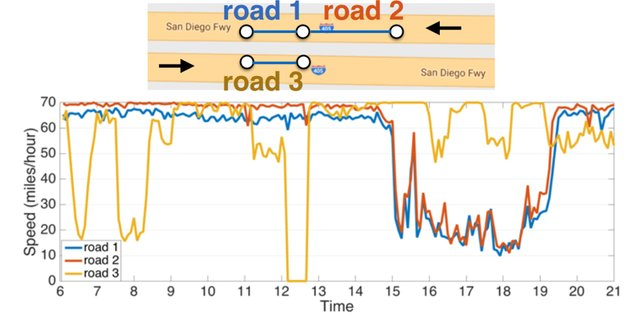
\includegraphics[width=.7\textwidth]{data.jpg}
\end{figure}
空间相关性主要由路网结构决定。对于监测的三条道路,其中,道路1与道路2位于同一条公路上,交通速度相似;道路1和道路3在公路的相反方向。虽然欧几里得距离很近,但交通速度差异较大。

\subsubsection{数据处理}
\begin{enumerate}
	\item 线性插值填充缺失值
	数据集中往往有大量的缺失值,会对训练造成影响。我们使用了线性插值法对缺失值进行填补。
	
	设缺失值前后两个时间片的观测值为$y_1$,$y_2$,则使用线性插值将其补为:
	$$
	\frac{y_1+y_2}{2}
	$$
	\item Z-score 归一化
	
	Z-Score归一化通过 $(x- \mu)/\sigma$将两组或多组数据转化为无单位的Z-Score分值,使得数据标准统一化,提高了数据可比性。
	
	\item 基于距离计算邻接矩阵
	
	邻接矩阵$A$代表了图的拓扑结构,而道路的长度决定了节点间相互影响的程度。将归一化后的距离作为邻接矩阵的值。
	
	$$
	w_{i j}=\left\{\begin{array}{l}
		\exp \left(-\frac{d_{i j}^{2}}{\sigma^{2}}\right), i \neq j \text { and } \exp \left(-\frac{d_{i j}^{2}}{\sigma^{2}}\right) \geq \epsilon \\
		0 \quad, \text { otherwise }
	\end{array}\right.$$
	
\end{enumerate}

\subsubsection{数据特征}
\begin{enumerate}
	\item 空间属性
	
	数据之间的相关性和相似性受节点之间的距离的影响,距离相近的数据之间的相似性更高。同时,一个位置的数据会受到周围和特定地点数据的影响,一般来说,距离越近,或地点之间的关联性越强,对该地点的数据的影响越大。
	
	\item 时间属性
	
	每个位置的数据按照时间顺序排列,形成时间属性。时空数据主要具有三种时间特性:
	\begin{itemize}
		\item 邻近性:相邻时间点的数据的相似性比相隔较远时间点的数据要高。
		\item 周期性:通常存在一定的周期模式,例如每日的高峰期和低峰期。
		\item 趋势性:即在更长的时间跨度上,数据的变化规律存在一定的趋势。
	\end{itemize}
\end{enumerate}

\subsubsection{预测问题}
对目标预测区域$t$时刻的交通流量定义无向图$G_t=(V_t,\varepsilon,W)$,其中$V_t$为$n$个节点的集合,表示区域内$n$个交通流的监测点,$\varepsilon$为边的集合,表示监测点间的连接,$W\in \mathbb{R}^{n\times n}$表示带权重的邻接矩阵。

预测任务为:建立一个函数$F(\cdot)$,将历史$H$个时间步的交通流量图中$n$个节点的流量向量$v_t$,映射到未来$M$个时间步的流量向量,即
$$
\hat v_{H+1},\dotsm, \hat v_{M}=F([v_1,\dotsm,v_H])
$$

\subsection{建立基本模型}
\subsubsection{图卷积网络}
由于卷积神经网络(CNN)无法处理非欧式数据,因此学者提出如何将卷积操作拓展到图数据上,开发了图卷积网络(Graph Convolutional Network)。其中一种方法基于图谱理论(spectral graph theory),利用图的傅里叶变换实现图卷积操作\cite{bib:two},如下式:
\begin{equation}\label{eq:a}
	\hat y = \sigma(Ug_{\theta}(\Lambda)U^Tx)
\end{equation}

记图的拉普拉斯矩阵(Laplacian matrix)为$L$,其中$U\in \mathbb{R}^{n\times n}$为$L$的特征向量,$\Lambda \in \mathbb{R}^{n\times n}$为$L$的特征值的对角矩阵,$g_{\theta}(\cdot)$表示要学习的参数的函数。

\subsubsection{基本模型}
基本模型参考了Yu, Yin和Zhu(2018)的研究\cite{bib:three}。模型的基本模块为STGCN模块,该模块结合了捕捉数据空间相关性和时间相关性的两种模块,整体结构如下图:
\begin{figure}[H]
	\centering
	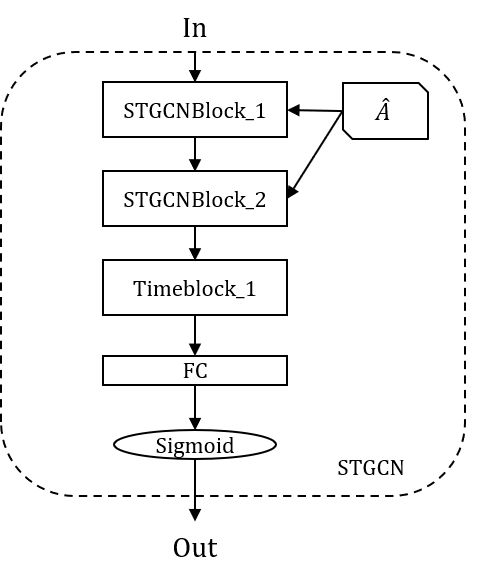
\includegraphics[width=.4\textwidth]{model1.png}
\end{figure}
其中,$\hat A$为图的邻接矩阵,将历史的图数据输入模型后,依次用两个STGCN模块充分提取数据的时间和空间特征,然后通过一个时间特征模块和全连接层,最终经过sigmoid激活函数后输出图未来若干时间步内的预测值。每个STGCN模块都由空间特征和时间特征组件构成。

\paragraph{空间特征组件}
空间特征组件采用图卷积操作捕捉流量拓扑图的空间相关性,为降低计算复杂度,提高效率,采用Chebyshev多项式\cite{bib:four}作为卷积核:
$$
g_{\theta}(\Lambda)=\sum_{k=0}^{K-1}\theta_k T_k(\tilde \Lambda)
$$
其中$T_k(\cdot)$是k阶的Chebyshev多项式,$\theta_k$是要训练的参数。$\tilde \Lambda $为归一化后的拉普拉斯矩阵特征值对角矩阵,
$$ \tilde{\Lambda} = 2\Lambda / \lambda_{max}-I$$

将该卷积核代入式\eqref{eq:a},则输出为
\begin{equation}
	y_{output}=\sigma(\sum_{k=0}^{K-1}\beta_k T_k(\tilde L)x)
\end{equation}
其中$\tilde{L}=2L/\lambda_{max}-I$。

\paragraph{时间特征组件}
时间特征组件结构采用一维卷积操作捕捉流量拓扑图的时间相关性,组件结构如下图所示:
\begin{figure}[H]
	\centering
	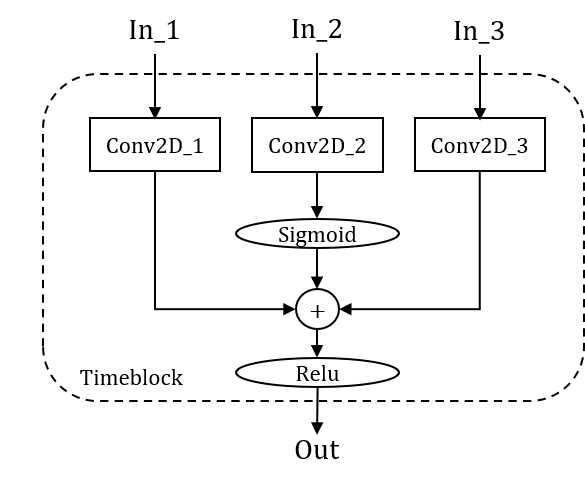
\includegraphics[width=.4\textwidth]{model3.png}
\end{figure}
将历史三个时刻的流量图$G_{t-2},G_{t-1},G_{t}$分别输入一个一维卷积层来提取时间相关性特征,其中由中间的一维卷积层输出的特征经过sigmoid函数处理,然后将三个特征整合,用ReLu激活函数后输出时间特征$T_{t+1}$。全过程如下式:
$$ T_{t+1} = \text{ReLU}(\Gamma *_{\mathcal{T}} G_{t-2}+\sigma(\Gamma *_{\mathcal{T}} G_{t-1})+\Gamma *_{\mathcal{T}} G_{t})$$
$\Gamma$为一维卷积核。

\paragraph{STGCN模块}
STGCN模块的具体结构如下图所示:
\begin{figure}[H]
	\centering
	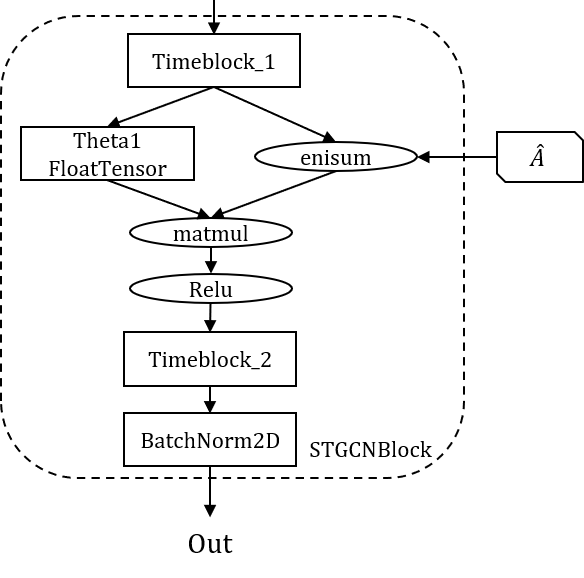
\includegraphics[width=.4\textwidth]{model2.png}
\end{figure}
主要由两个时间特征组件和一个空间特征组件组成。输入的历史流量图数据依次经过交错排列的时间和空间特征组件,得到时空相关性特征,对提取的特征进行批处理操作后输出。

\subsection{模型实验}
\subsubsection{实验设置}
\paragraph{超参数设置}
学习率为0.01,时间片间隔为5分钟,预测时间长度为5分钟(即预测下5分钟的交通情况)。

\paragraph{评价指标}
我们使用在交通预测中常用的三个指标对模型性能进行评价。
\begin{itemize}
	\item Mean Absolute Error(MAE),表示成对观测值之间误差的量度。
	$$\operatorname{MAE}=\frac{\sum_{i=1}^{n}\left|\hat y_{i}-y_{i}\right|}{n}=\frac{\sum_{i=1}^{n}\left|e_{i}\right|}{n}$$
	
	\item Mean Absolute Percentage Error(MAPE),为每个绝对误差的和除以实际值。
	$$\mathrm{MAPE}=\frac{1}{n} \sum_{t=1}^{n}\left|\frac{\hat y_{t}-y_{t}}{y_{t}}\right|$$
	
	\item Root Mean Squared Error (RMSE),为误差平方平均值的平方根。
	$$ \mathrm{RMSE}=\sqrt{\dfrac{1}{n}\sum_{i=1}^n(\hat y_i-y_i)^2}
	$$
	
\end{itemize}

\subsubsection{单步实验结果}
\begin{table}[H]
	\begin{center}
		\begin{tabular}{cc}
			\toprule[1.5pt]
			\multicolumn{1}{m{4cm}}{\centering 指标}
			&\multicolumn{1}{m{4cm}}{\centering 实验值}\\
			\midrule[1.0pt]
			MAE  & 3.58\\
			MAPE  & 11.23\\
			RMSE  & 7.76\\
			\bottomrule[1.5pt]
		\end{tabular}\label{tb:notation}
	\end{center}
\end{table}

\begin{figure}[H]
	\centering
	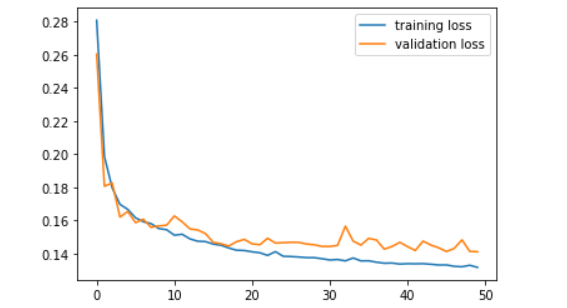
\includegraphics[width=0.7\linewidth]{results}
	\label{fig:results}
\end{figure}

模型在各项指标上都取得了较为满意的结果,MAPE和RMSE与同类模型相比较都有明显优势,体现出了图卷积神经网络的强大。但MAPE明显偏高,说明对于异常值的处理不够准确,无法捕捉因天气等产生的异常情况。

\section{下阶段研究计划}
\begin{enumerate}
	\item 继续搜集和阅读交通预测问题和图神经网络的相关文献,参考前人的研究模型和实验结果,考虑如何改进模型:
	\begin{enumerate}
		\item 基本模型架构设计,如引入注意力机制等;
		\item 如何调整模型参数。制定相应的实验方案,验证改进方案,减小预测误差,提高模型的预测精确度和鲁棒性。
	\end{enumerate}
	\item 考虑如何对外部因素建模,在预测模型中加入外部因素(如天气、节假日等)对交通流量的影响的特征捕捉。制定外部因素模型建立方案和相应的实验方案,优化基本模型,增强模型的现实性和普适性。
	\item 进行建模收尾工作,实现高效的数据可视化,讨论预测结果的潜在价值和模型的现实意义。
	\item 以研究报告和学术论文等方式总结研究成果。
\end{enumerate}

\begin{thebibliography}{9}%宽度9
	\bibitem{bib:five}Li, Y. , Yu, R. , Shahabi, C. , \& Liu, Y. . (2017). Diffusion convolutional recurrent neural network: data-driven traffic forecasting.
	\bibitem{bib:one}Zhang, J. , Zheng, Y. , Qi, D. , Li, R. , \& Yi, X. . (2016). DNN-based prediction model for spatio-temporal data. the 24th ACM SIGSPATIAL International Conference. ACM.
	\bibitem{bib:two}Bruna, J. , Zaremba, W. , Szlam, A. , \& Lecun, Y. . (2013). Spectral networks and locally connected networks on graphs. Computer ence.
	\bibitem{bib:three}Yu, B. , Yin, H. , \& Zhu, Z. . (2018). Spatio-Temporal Graph Convolutional Networks: A Deep Learning Framework for Traffic Forecasting. Twenty-Seventh International Joint Conference on Artificial Intelligence IJCAI-18.
	\bibitem{bib:four}Hammond, D. K. , Vandergheynst, P. , \& Rémi Gribonval. (2011). Wavelets on graphs via spectral graph theory. Applied \& Computational Harmonic Analysis, 30(2), 129-150.
\end{thebibliography}

\end{document}